\documentclass[letterpaper,12pt]{book}
%Interlineado 1.5
%\renewcommand{\baselinestretch}{1.5}
\usepackage[utf8]{inputenc}
%Para evitar problemas de compatibilidad con el package tikz
\usepackage[spanish,es-noshorthands,es-tabla]{babel}
%\usepackage{subfigure}
%\usepackage[spanish,onelanguage]{algorithm}
%\usepackage{algorithmic}
\usepackage{algpseudocode}
\usepackage[spanish,onelanguage,ruled,linesnumbered]{algorithm2e} %ruled, vlined
\usepackage{listings}
\usepackage{amsthm}
\usepackage{textcomp}
\usepackage{multicol}
\usepackage{float}
\usepackage{url}
\usepackage{enumerate}
\usepackage{enumitem}
\usepackage{newlfont}
\usepackage{psfrag}
\usepackage{charter}
\usepackage{setspace}
\usepackage{longtable}
%\usepackage{subfigure}
\usepackage[dvips]{epsfig}
\usepackage[centertags]{amsmath}
\usepackage{newlfont}
\usepackage{psfrag}
\usepackage{textcomp}
\usepackage{framed}
\usepackage{verbatim}
\usepackage{multirow}
\usepackage{graphicx}
\usepackage[font=footnotesize]{caption}
\usepackage[font=scriptsize]{subcaption}
\usepackage{appendix}
%\usepackage{biblatex}

\usepackage[table]{xcolor}

\usepackage{fancyhdr}
\pagestyle{fancy}
\thispagestyle{plain}
\fancyhead[H]{} %header vacio
\renewcommand{\headrulewidth}{0pt}


%fonts matematicos
\usepackage{amsfonts}
\usepackage{amssymb}
\usepackage{amsmath}

%Diagramas
\usepackage{tikz}
\usetikzlibrary{positioning,calc,arrows,snakes,patterns}

%links
\usepackage{color}
 \usepackage{hyperref}
 \hypersetup{
     colorlinks=true,
     linktoc=section,
     linkcolor=red,
     citecolor=blue,
 }


\usepackage[top=2.5cm,bottom=2.5cm,left=4cm,right=2.5cm,asymmetric]{geometry}

\setlength{\parindent}{0pt}

%Profundidad Tabla de Contenidos
\setcounter{tocdepth}{4}
\setcounter{secnumdepth}{4}

% CAPITULO 1 NOMBRE
\usepackage{titletoc}     % http://ctan.org/pkg/titletoc
\titlecontents{chapter}   % <section-type>
  [0pt]% <left>
  {\addvspace{1em}}% <above-code>
  {\bfseries\chaptername\ \thecontentslabel\quad}% <numbered-entry-format>
  {}% <numberless-entry-format>
  {\bfseries\hfill\contentspage}% <filler-page-format>

\usepackage{apacite}

\renewcommand{\baselinestretch}{1.3}

\begin{document}
  \renewcommand{\BOthers}[1]{et al.\hbox{}}

  %Cambio de titulos
  \renewcommand*\contentsname{Índice General}
  \renewcommand*\listfigurename{Índice de Figuras}
  \renewcommand*\listtablename{Índice de Tablas}
  \renewcommand*\listalgorithmcfname{Índice de Algoritmos}
  %\renewcommand\spanishtablename{Tabla}
  \renewcommand{\appendixtocname}{Apéndices}
  \renewcommand{\appendixpagename}{Apéndices}

  %Definiciones
  \newcounter{defctr}
  \newenvironment{definition}{
    \refstepcounter{defctr}
    \begin{framed}
    \textbf{Definición \thedefctr}
    \newline
  }{\end{framed} \par \bigskip }
  \numberwithin{defctr}{chapter}

  \definecolor{light-gray}{gray}{0.95}
  \definecolor{light-gray-2}{gray}{0.8}


  % Estructura de contenidos para presentar
  % el trabajo de titulo

  \let\cleardoublepage\clearpage

  \thispagestyle{empty}
\begin{titlepage}

\begin{center}

\vspace*{-1in}
\begin{figure}[htb]
  \begin{flushleft}
    
\includegraphics[width=10cm]{./figuras/logo_informatica.jpg}
  \end{flushleft}
\end{figure}

{\setstretch{1.5}
\vspace*{4cm}
\textbf{ \large{TITULO DE LA TESIS}} \\
\vspace*{2.0in}
}

\normalsize{por} \\
\vspace*{0.1in}
\normalsize{NOMBRE1 NOMBRE2 APELLIDO1 APELLIDO2} \\
\vspace*{1.3in}
\normalsize{Trabajo de Título presentado a la  \\ Facultad de Ingeniería de la Universidad Católica de Temuco  \\ Para Optar al Título de Ingeniero Civil en Informática \\}
\vspace*{0.5in}
\normalsize{- Temuco, MES AÑO -}
\end{center}

\end{titlepage}

  %\input{comision.tex}
  
\thispagestyle{empty}
\begin{titlepage}

{\setstretch{1.0}
\begin{center}
\vspace*{-1in}
\begin{figure}[htb]
\begin{center}

\includegraphics[width=8cm]{./figuras/logo_informatica.jpg}
\end{center}
\end{figure}

\vspace*{0.2in}
\textbf{ \normalsize{INFORME TRABAJO DE TÍTULO}} \\
\vspace*{0.2in}
\begin{flushleft}
\textbf{ \normalsize{TÍTULO:}} \hspace*{0.2in} \textbf{ \textit{ \normalsize{``TITULO DE LA TESIS''.}}}
\end{flushleft}
\vspace*{0.1in}
\begin{flushleft}
\textbf{ \normalsize{ALUMNO:}} \hspace*{0.2in} \textbf{ \normalsize{NOMBRE1 NOMBRE2 APELLIDO1 APELLIDO2}}
\end{flushleft}
\vspace*{0.3in}

\begin{flushleft}

\hspace{1cm} En mi calidad de Profesor Guía y luego de haber analizado y revisado el informe de Trabajo de Título puedo concluir lo siguiente:

\begin{list}{$\bullet$}{}
  \item Reportes del profesor
\end{list}

\hspace{1cm} De acuerdo a las previas observaciones califico el presente informe con \textbf {nota 7.0 (siete coma cero)}.
\end{flushleft}

\vspace*{0.5in}

\begin{flushright}
 \rule{65mm}{0.2mm}\\
\end{flushright}
\vspace*{-0.1in}
 \hspace*{3.5in} \textbf{Nombre Profesor Guia} \\
 \hspace*{3.5in} \textbf{Profesor Guía}

\vspace*{0.6in}

\begin{flushleft}
  Temuco, DIA de MES de AÑO.
\end{flushleft}

\end{center}
}
\end{titlepage}

  
\thispagestyle{empty}
\begin{titlepage}

{\setstretch{1.0}
\begin{center}
\vspace*{-1in}
\begin{figure}[htb]
\begin{center}

\includegraphics[width=8cm]{./figuras/logo_informatica.jpg}
\end{center}
\end{figure}

\vspace*{0.2in}
\textbf{ \normalsize{INFORME TRABAJO DE TÍTULO}} \\
\vspace*{0.2in}
\begin{flushleft}
\textbf{ \normalsize{TÍTULO:}} \hspace*{0.2in} \textbf{ \textit{ \normalsize{``Implementación de una plataforma de APIs centralizada para desarrolladores en base a micro servicios, utilizando Node Red, Kubernetes y React , bajo la plataforma Google Cloud Platform.''.}}}
\end{flushleft}
\vspace*{0.1in}
\begin{flushleft}
\textbf{ \normalsize{ALUMNO:}} \hspace*{0.2in} \textbf{ \normalsize{Alfonso Andres Duarte Belmar}}
\end{flushleft}
\vspace*{0.3in}

\begin{flushleft}

\hspace{1cm} En mi condición de Profesor Informante presento el informe de calificación del Trabajo de Título del alumno
  Alfonso Andres Duarte Belmar bajo las siguientes observaciones:

\begin{list}{$\bullet$}{}
  \item Lo que dice el profesor informante.
\end{list}

\hspace{1cm} De acuerdo a estas consideraciones califico el desarrollo de éste Trabajo de Título con \textbf {nota 7.0 (siete coma cero)}.
\end{flushleft}

\vspace*{0.5in}

\begin{flushright}
 \rule{65mm}{0.2mm}\\
\end{flushright}
\vspace*{-0.2in}
 \hspace*{3.5in} \textbf{Nombre Profesor Informante} \\
 \hspace*{3.5in} \textbf{Profesor Informante}

\vspace*{0.6in}

\begin{flushleft}
Temuco, 31 de Diciembre de 2021.
\end{flushleft}

\end{center}
}
\end{titlepage}

  \thispagestyle{empty}
\begin{titlepage}
  {\setstretch{1.0}
  \vspace*{6.0in}
  \begin{flushright}

     Deseo  dedicar esta tesis a mi madre Victoria, que con su amor, paciencia y esfuerzo me ha permitido llegar a cumplir hoy un sueño más, muchas gracias por inculcar en mí, el ejemplo de esfuerzo y perseverancia, de no temer las adversidades porque Dios está conmigo siempre. 
     
     \hfill
    
    A mis tías Marta, Violeta y Nilda, por su cariño y apoyo incondicional, durante todo este proceso, por estar conmigo en todo momento gracias. Gracias a sus oraciones, consejos y palabras de aliento, que hicieron de mí una mejor persona y de una u otra forma me acompañaran en todos mis sueños y metas futuras.
    
     \hfill
    
    De todo corazón mil gracias, siempre las llevare en mi corazón.
    
       \hfill
    
    Andres Duarte Belmar

  \end{flushright}
  }
\end{titlepage}
  \thispagestyle{empty}
\begin{titlepage}
\begin{center}
\section*{AGRADECIMIENTOS}
\end{center}

%\newgeometry{margin=1cm}

\begin{flushleft}

  Aquí van los agradecimientos

\end{flushleft}
\end{titlepage}



  % Indice
  % Numeracion romana
  \pagenumbering{Roman}

  \tableofcontents
  \addcontentsline{toc}{chapter}{Índice General}
  \cleardoublepage

  \phantomsection
  \addcontentsline{toc}{chapter}{Índice de Figuras}
  \listoffigures
  \cleardoublepage

  \phantomsection
  \addcontentsline{toc}{chapter}{Índice de Tablas}
  \listoftables
  \cleardoublepage

  \phantomsection
  \addcontentsline{toc}{chapter}{Índice de Algoritmos}
  \listofalgorithms
  \cleardoublepage

  % Resumen
  \chapter*{Resumen} % si no queremos que añada la palabra "Capitulo"

El objetivo primordial de este trabajo es implementar una plataforma  de apis centralizada, basada en una arquitectura de micro servicios en la nube. En el presente informe hablaremos de cuales son la  ventajas y desventajas de una arquitectura de micro servicios implementada en ambientes cloud, enfocando además las ventajas de este tipo de implementación, frente a una monolítica. La contruccion de las  APIs implementadas utilizaron como puente de conexión a Node-Red, el cual es una herramienta de programación para conectar APIs y servicios en línea. Este proyecto se realizo bajo la plataforma Google Cloud Plataform(GCP) y serán desplegadas en producción en ambientes contenerizados utilizando Docker y Kubernetes. En resumen trataremos los principales paradigamas en el desarrollo de apis basados en micro servicios en ambientes cloud. 

\hfill

Palabras Clave: APIs, Microservicios, Contenedores, Docker, Kubernetes, Cluster, Node-Red, GCP.

\addcontentsline{toc}{chapter}{Resumen}
\clearpage

\chapter*{Abstract}

The primary goal of this work is to implement a centralized apis platform based on a cloud microservices architecture. In this report we will discuss the advantages and disadvantages of a microservices architecture implemented in cloud environments, focusing also on the advantages of this type of implementation, versus a monolithic one. The construction of the implemented APIs used Node-Red as a connection bridge, which is a programming tool to connect APIs and online services. This project was done under the Google Cloud Platform (GCP) and will be deployed in production in containerized environments using Docker and Kubernetes. In summary we will discuss the main paradigms in the development of apis based on microservices in cloud environments. 

\hfill

Keywords: APIs, Microservices, Containers, Docker, Kubernetes, Cluster, Node-Red, GCP.

\addcontentsline{toc}{chapter}{Abstract}

  \cleardoublepage


  % Capitulos del trabajo
  % Uso de numeracion Arabica
  \pagenumbering{arabic}

  
%% CAPÍTULO 1 %%
\chapter{Introducción}

  %% SECCIÓN %%
  \section{Problema}

 Hoy en día los desarrollos de software especializados en apis son complejos, ya que normalmente se realizaban basándose en base a una arquitectura monolítica, la cual es difícil de  mantener y escalar. En la actualidad se observa como las empresas están decantándose por arquitecturas de microservicios, ya que les otorga muchos beneficios como son estandarización, escalabilidad, mantenimiento y agilidad.
La forma de aplicar los microservicios no es difícil, ya que actualmente existen variadas tecnologías y frameworks que permiten su implementación, además los despliegues se pueden realizar utilizando tecnologías basadas en contenedores tales como Docker y Kubernetes, entre otros. 

\hfill

El problema  que actualmente tienen miles de desarrolladores de Chile,  tanto para trabajo, como para proyectos de desarrollo personal, es que deben  consumir APIs de diferentes fuentes públicas.  Esto genera en muchos casos, que deban recurrir uno por uno, a servicios que no poseen una documentación estandarizada acorde a los tiempos de hoy. Para solventar este problema se implementa, mediante una plataforma de APIs centralizada, la cual se encargará de controlar toda la comunicación y seguridad de los micro servicios, que actualmente están esparcidos en la red. De esta manera se reduce la complejidad que se tiene al implementar este tipo de arquitectura, en donde se necesita tener una pasarela de APIs para los desarrolladores del país.

%   \begin{figure}[!htb]
%     \begin{center}
%     	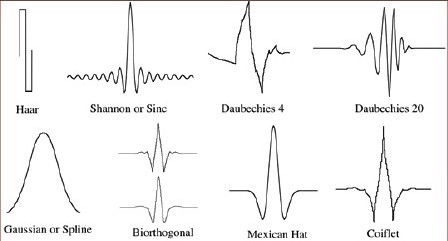
\includegraphics[width=15cm]{./figuras/wavelets.jpg}
%     	\caption{Ejemplos de figura}
%     \end{center}
%     \label{fig:figura}
%   \end{figure}



  %% SECCIÓN %%
  \section{Estado del Arte}
  





  % Bibliografia - Referencias
  \cleardoublepage
  \addcontentsline{toc}{chapter}{Bibliografía}
  \bibliographystyle{apacitex}
  \bibliography{referencias}

  % Apendices
  \cleardoublepage
\addappheadtotoc
\appendixpage
\appendix
  \chapter{Codigos} \label{apenA}
    \section{Codigo Node-Red}
    \section{Codigo React}
    \section{Yaml}

	\clearpage


\end{document}
